\documentclass{article}
\usepackage[a4paper, total={6in, 8in}]{geometry}
\usepackage{graphicx} % Required for inserting images
\usepackage{algorithm}
\usepackage{algpseudocode}
\usepackage{listings}
\usepackage{csquotes}
\usepackage{xcolor}

\definecolor{codegreen}{rgb}{0,0.6,0}
\definecolor{codegray}{rgb}{0.5,0.5,0.5}
\definecolor{codepurple}{rgb}{0.58,0,0.82}
\definecolor{backcolour}{rgb}{0.95,0.95,0.92}

\lstdefinestyle{mystyle}{
    backgroundcolor=\color{backcolour},   
    commentstyle=\color{codegreen},
    keywordstyle=\color{magenta},
    numberstyle=\tiny\color{codegray},
    stringstyle=\color{codepurple},
    basicstyle=\ttfamily\footnotesize,
    breakatwhitespace=false,         
    breaklines=true,                 
    captionpos=b,                    
    keepspaces=true,                 
    %numbers=left,                    
    numbersep=5pt,                  
    showspaces=false,                
    showstringspaces=false,
    showtabs=false,                  
    tabsize=2
}

\lstset{style=mystyle}
\title{Latex sample codes for good formating}
\author{Gaurav kumar}
\date{July 2023}

\begin{document}

\maketitle

As I recently heard someone say:

\begin{displayquote}
\centering
``Life is hard. But it's harder when you are dumb."
\end{displayquote}

Below mentioned writing and formatting guidelines are not just for latex but for a general purpose writing/presentation. Latex only makes it easier to implement these guidelines. No one is perfect at anything and there is always room for improvement. These are some of the writing tips I found useful for myself. Probably you will too!

\section*{Some rules of thumb for good writing}
\begin{enumerate}
    \item Be concise. It is not an achievement to write a very long document. 
    \item Be kind to others. Write your thoughts clearly so that the next person doesn't struggle to understand it. If you want someone's help/opinion on something (case with internal reports/presentations etc.) or want them to adopt your method or opinion (case in journal/conference publications), you don't want to scare them with a long document or some very difficult to read material. 
    \item Be generous in describing your figures, tables, algorithms, code listing etc.
    \item Don't use jargons. If you use acronyms or abbreviations, please define them at the first instance of appearance.
    \item Don't randomly capitalize words for emphasis. It makes the document hard to read and it is distracting. If you need to emphasize something, properly use the language, especially punctuations to do so. Only first letters of the sentences should be capitalized except for proper nouns and some acronyms.
    \item Never start a subsection without describing what the section is about. \emph{e.g.}

    \begin{section}{A section}
        This is a section. Here we'll talk about two different things. Hence, there are two subsections.
        \begin{subsection}{A subsection}
            This is subsection 1.1.
        \end{subsection}
        \begin{subsection}{Another subsection}
            This is subsection 1.2.
        \end{subsection}
    \end{section}


\item Figures should always have descriptive captions. It should not be like Figure 1 or Figure 1.1. 
\begin{figure}[H]
\centering
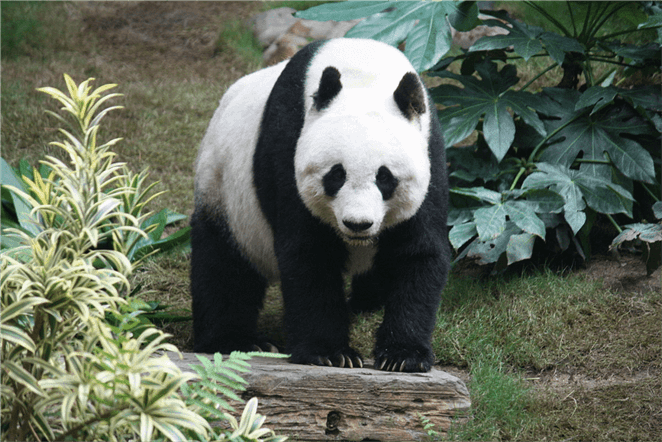
\includegraphics[width=0.9\textwidth]{figures/fig1.png}
\caption{An example of how to insert a figure in latex. This is a panda.}
\end{figure}

If you have multiple subfigures, combine them together and insert as one figure shown below. You can use Inkscape or some similar softwares to work on your figures.

\begin{figure}[H]
\centering
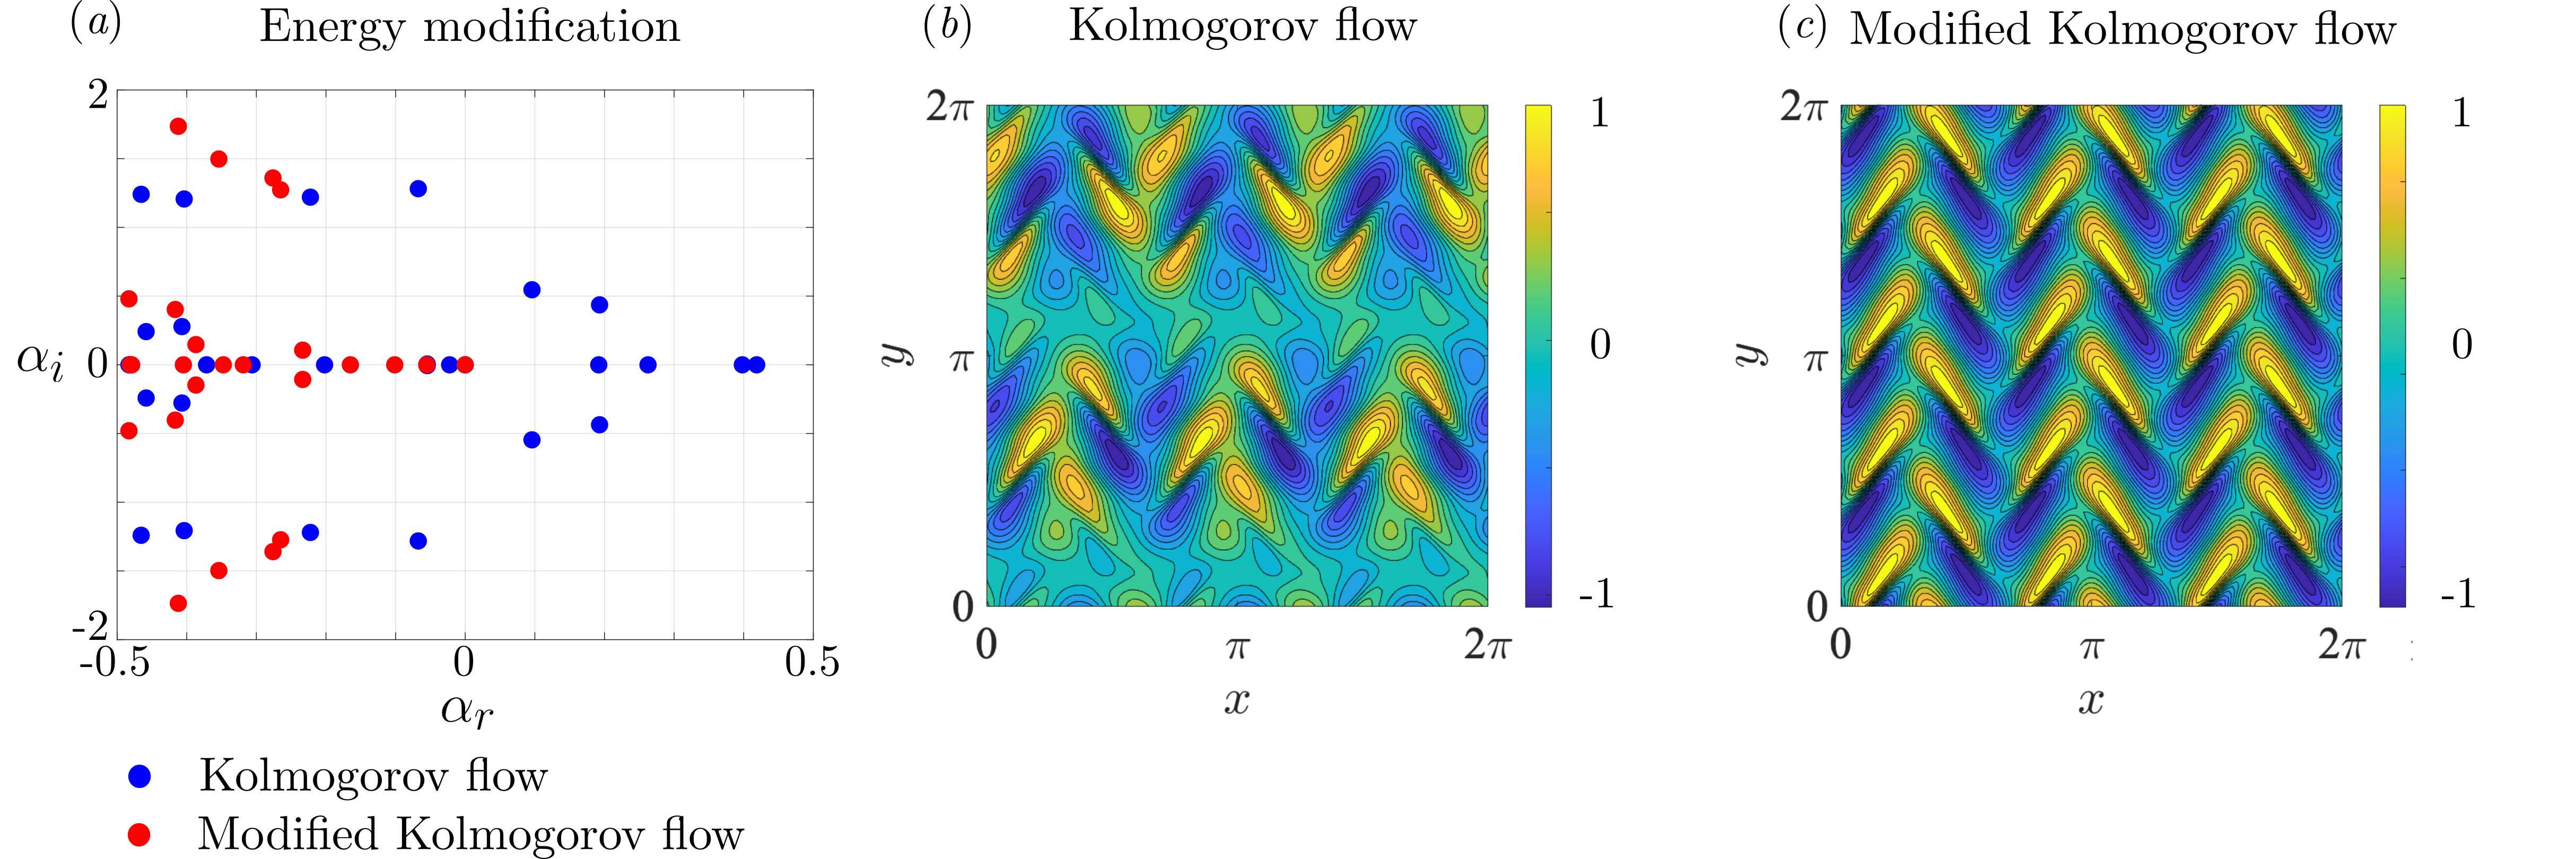
\includegraphics[width=\textwidth]{figures/EigenValues.png}
\caption{A example of a figure with three subfigures.}
\end{figure}

The text in the figures should always be legible. Graphs should always have axes labels, tick marks, legends and title (if necessary). Lines and markers should have easily distinguishable colours, linestyles and marker sizes. Don't clutter a single plot with too many lines. Split into multiple figure if you have too much data to show.

\item Tables should always have descriptive captions. It should not be like Table 1 or Table 1.1. 
\begin{table}[H]
\centering
\caption{A table with three rows and three columns.} \vspace{0.1in}
\begin{tabular}{ |c|c|c| } 
 \hline
 cell1 & cell2 & cell3 \\ \hline
 cell4 & cell5 & cell6 \\ 
 cell7 & cell8 & cell9 \\ 
 \hline
\end{tabular}
\end{table}

\item How to insert an algorithm in latex?\\
\begin{algorithm}
\caption{An algorithm with caption}\label{alg:cap}
\begin{algorithmic}
\Require $n \geq 0$
\Ensure $y = x^n$
\State $y \gets 1$
\State $X \gets x$
\State $N \gets n$
\While{$N \neq 0$}
\If{$N$ is even}
    \State $X \gets X \times X$
    \State $N \gets \frac{N}{2}$  \Comment{This is a comment}
\ElsIf{$N$ is odd}
    \State $y \gets y \times X$
    \State $N \gets N - 1$
\EndIf
\EndWhile
\end{algorithmic}
\end{algorithm}

\item How to insert a code in latex?\\
\begin{lstlisting}[language=bash, caption=An example of code listing]          % Start your code-block

# = = = = = = = = = = = = = = = = = = = = = = = = = = = = = = = = = = = =
# 2 d grid with a minimal spanwise thickness
# = = = = = = = = = = = = = = = = = = = = = = = = = = = = = = = = = = = =
# Base mesh resolution
DEFINE DELTA =0.16
DEFINE MAX_REFINEMENT_LEVEL=3
DEFINE LZ =(0.5*$(DELTA)/ pow (2 ,$(MAX_REFINEMENT_LEVEL)))
# Define the surface and point seeding
PART SURF = SIMPLE_BOX 0 25 0 4 -$(LZ) $(LZ)
# Base mesh resolution
HCP_DELTA $(DELTA)
# Refinement windows are specified here . y0 is the zone representing
the plate .
HCP_WINDOW FAZONE y0 LEVEL =$(MAX_REFINEMENT_LEVEL) N=4 NLAYERS=4 ,4
# Number of smoothing iterations
NSMOOTH 10
# ================
# viz
# ================
\end{lstlisting}

\item This is work in progress. More will be added in time.
\end{enumerate}
\end{document}
